\documentclass[]{article}
\usepackage{lmodern}
\usepackage{amssymb,amsmath}
\usepackage{ifxetex,ifluatex}
\usepackage{fixltx2e} % provides \textsubscript
\ifnum 0\ifxetex 1\fi\ifluatex 1\fi=0 % if pdftex
  \usepackage[T1]{fontenc}
  \usepackage[utf8]{inputenc}
\else % if luatex or xelatex
  \ifxetex
    \usepackage{mathspec}
  \else
    \usepackage{fontspec}
  \fi
  \defaultfontfeatures{Ligatures=TeX,Scale=MatchLowercase}
\fi
% use upquote if available, for straight quotes in verbatim environments
\IfFileExists{upquote.sty}{\usepackage{upquote}}{}
% use microtype if available
\IfFileExists{microtype.sty}{%
\usepackage{microtype}
\UseMicrotypeSet[protrusion]{basicmath} % disable protrusion for tt fonts
}{}
\usepackage[margin=1in]{geometry}
\usepackage{hyperref}
\hypersetup{unicode=true,
            pdftitle={Data Management Plan for the Study Do Reputable Open Access Journals Require Open Data Sharing?},
            pdfauthor={Gail Clement and Tom Morrell},
            pdfborder={0 0 0},
            breaklinks=true}
\urlstyle{same}  % don't use monospace font for urls
\usepackage{longtable,booktabs}
\usepackage{graphicx,grffile}
\makeatletter
\def\maxwidth{\ifdim\Gin@nat@width>\linewidth\linewidth\else\Gin@nat@width\fi}
\def\maxheight{\ifdim\Gin@nat@height>\textheight\textheight\else\Gin@nat@height\fi}
\makeatother
% Scale images if necessary, so that they will not overflow the page
% margins by default, and it is still possible to overwrite the defaults
% using explicit options in \includegraphics[width, height, ...]{}
\setkeys{Gin}{width=\maxwidth,height=\maxheight,keepaspectratio}
\IfFileExists{parskip.sty}{%
\usepackage{parskip}
}{% else
\setlength{\parindent}{0pt}
\setlength{\parskip}{6pt plus 2pt minus 1pt}
}
\setlength{\emergencystretch}{3em}  % prevent overfull lines
\providecommand{\tightlist}{%
  \setlength{\itemsep}{0pt}\setlength{\parskip}{0pt}}
\setcounter{secnumdepth}{0}
% Redefines (sub)paragraphs to behave more like sections
\ifx\paragraph\undefined\else
\let\oldparagraph\paragraph
\renewcommand{\paragraph}[1]{\oldparagraph{#1}\mbox{}}
\fi
\ifx\subparagraph\undefined\else
\let\oldsubparagraph\subparagraph
\renewcommand{\subparagraph}[1]{\oldsubparagraph{#1}\mbox{}}
\fi

%%% Use protect on footnotes to avoid problems with footnotes in titles
\let\rmarkdownfootnote\footnote%
\def\footnote{\protect\rmarkdownfootnote}

%%% Change title format to be more compact
\usepackage{titling}

% Create subtitle command for use in maketitle
\providecommand{\subtitle}[1]{
  \posttitle{
    \begin{center}\large#1\end{center}
    }
}

\setlength{\droptitle}{-2em}

  \title{Data Management Plan for the Study \emph{Do Reputable Open Access
Journals Require Open Data Sharing?}}
    \pretitle{\vspace{\droptitle}\centering\huge}
  \posttitle{\par}
    \author{Gail Clement and Tom Morrell}
    \preauthor{\centering\large\emph}
  \postauthor{\par}
      \predate{\centering\large\emph}
  \postdate{\par}
    \date{August 2, 2018}


\begin{document}
\maketitle

{
\setcounter{tocdepth}{2}
\tableofcontents
}
\begin{center}\rule{0.5\linewidth}{\linethickness}\end{center}

\hypertarget{introduction}{%
\section{Introduction}\label{introduction}}

This study analyzes the submission requirements of the most reputable
open access journals to determine the prevalence and characteristics of
data sharing policies. This question is an important one for
21\textsuperscript{st} century authors and readers because open data
sharing is seen as a key component of open and more trusted scientific
record.

\hypertarget{purpose-of-this-study}{%
\subsection{Purpose of this Study}\label{purpose-of-this-study}}

This study investigates whether the \textbf{most reputable Open Access
journals} have data sharing polices and the characteristics of those
policies. These policies require authors, in some fashion, to openly
disseminate the data and software underlying their published articles.
Our investigation builds on the recent work of Castro et al (2017) who
assessed the prevalence and characteristics of data sharing policies
from randomly-selected, English-language, open access journals. Their
findings reveal that only a small minority of these journals have data
sharing policies. These findings -- which are consistent with those of
other studies (see for example, ``Reproducible and Reusable Research:
Are Journal Data Sharing Policies Meeting the Mark?'' n.d.) -- may be
skewed because of the authors' rules of inclusion and
exclusion.\footnote{in particular, the choice to include open access
  journals merely because of their use of the Open Journal Systems (OJS)
  hosting platform; the choice to exclude non\_English language journals}

\hypertarget{methodology}{%
\subsection{Methodology}\label{methodology}}

In this study, we will include only the most reputable open access
journals in our assessment of journal sharing policies, reglardless of
language. We will analyze all journals that have attained the Seal of
Approval from the \href{http://doaj.org}{\emph{\textbf{Directory of Open
Access Journals, DOAJ}}} (shown below). We will apply the same coding
framework devised by Castro et al. (2017) to the DOAJ Seal journals. We
contend that a more rigorously screened population of open access
journals, regardles of language, will yield a more accurate and
reproducible set of findings than those published from Castro et al.
(2017).

Moreover, the DOAJ Seal journals do include over 200 non-English
language journals that merit analysis in this study. Excluding these
from the analysis represents cultural bias that undermines reliable
research. The following plot of DOAJ Seal Journals by Country indicates
the problem.

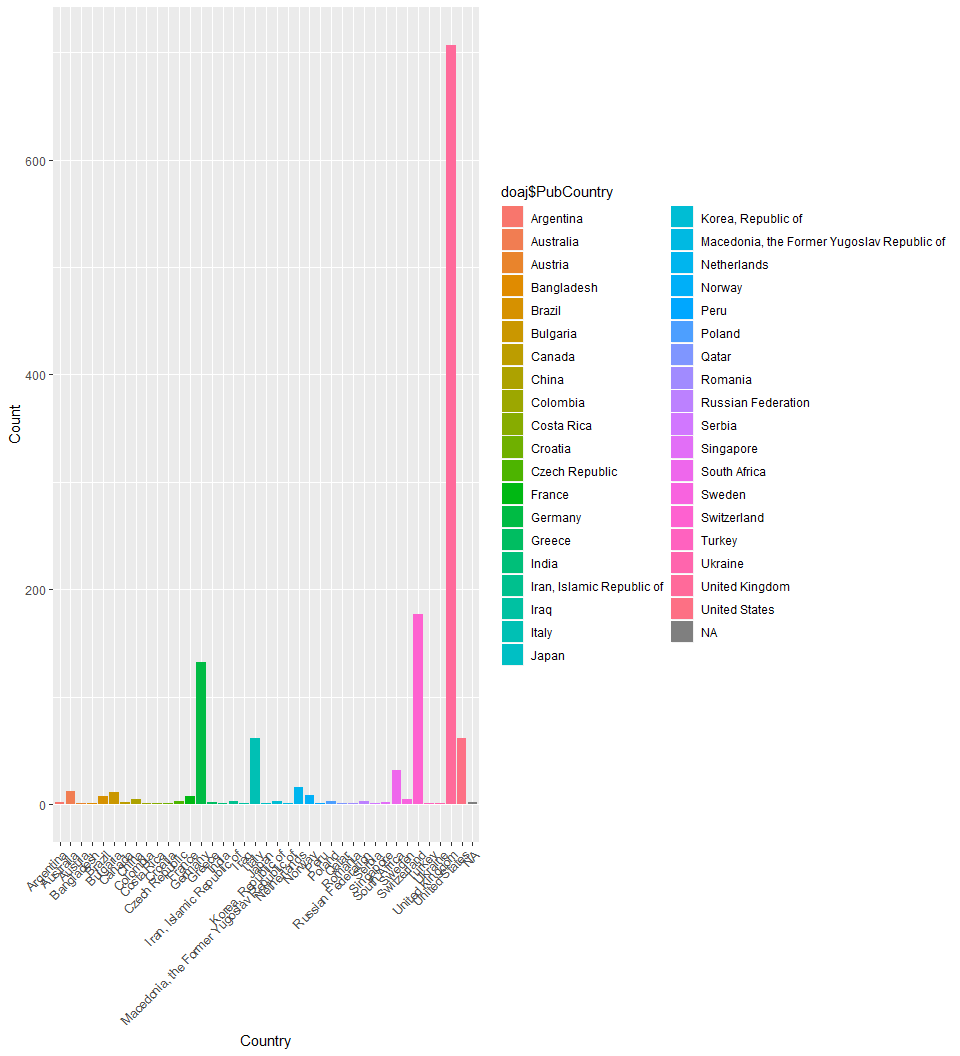
\includegraphics{Base_2013_1_files/figure-latex/plot_country-1.pdf}

A sample of the \texttt{doaj\_seal.csv} data set is shown below.

\begin{longtable}[]{@{}llllllrlllrlll@{}}
\caption{A Table of the first 4 rows of the DOAJ Seal
data.}\tabularnewline
\toprule
JnlTitle & Publisher & PubCountry & Fee & WaiverPolicy & Identifiers &
FirstYear & Language & ReviewProcess & Plagiarism & Sub2Pub & JnlLicense
& AuthorCopyright & DOAJ\_Seal\tabularnewline
\midrule
\endfirsthead
\toprule
JnlTitle & Publisher & PubCountry & Fee & WaiverPolicy & Identifiers &
FirstYear & Language & ReviewProcess & Plagiarism & Sub2Pub & JnlLicense
& AuthorCopyright & DOAJ\_Seal\tabularnewline
\midrule
\endhead
Archives Animal Breeding & Copernicus Publications & Germany & No & Yes
& DOI & 1999 & English & Peer review & Yes & 13 & CC BY & TRUE &
Yes\tabularnewline
Bothalia: African Biodiversity \& Conservation & AOSIS & South Africa &
No & NA & DOI & 2014 & English & Double blind peer review & Yes & 12 &
CC BY & TRUE & Yes\tabularnewline
Geographica Helvetica & Copernicus Publications & Germany & No & Yes &
DOI & 1946 & English, French, German, Italian & Double blind peer review
& Yes & 53 & CC BY & TRUE & Yes\tabularnewline
Hereditas & BioMed Central & United Kingdom & Yes & Yes & DOI & 2005 &
English & Blind peer review & Yes & 6 & CC BY & TRUE &
Yes\tabularnewline
\bottomrule
\end{longtable}

\hypertarget{results}{%
\section{Results}\label{results}}

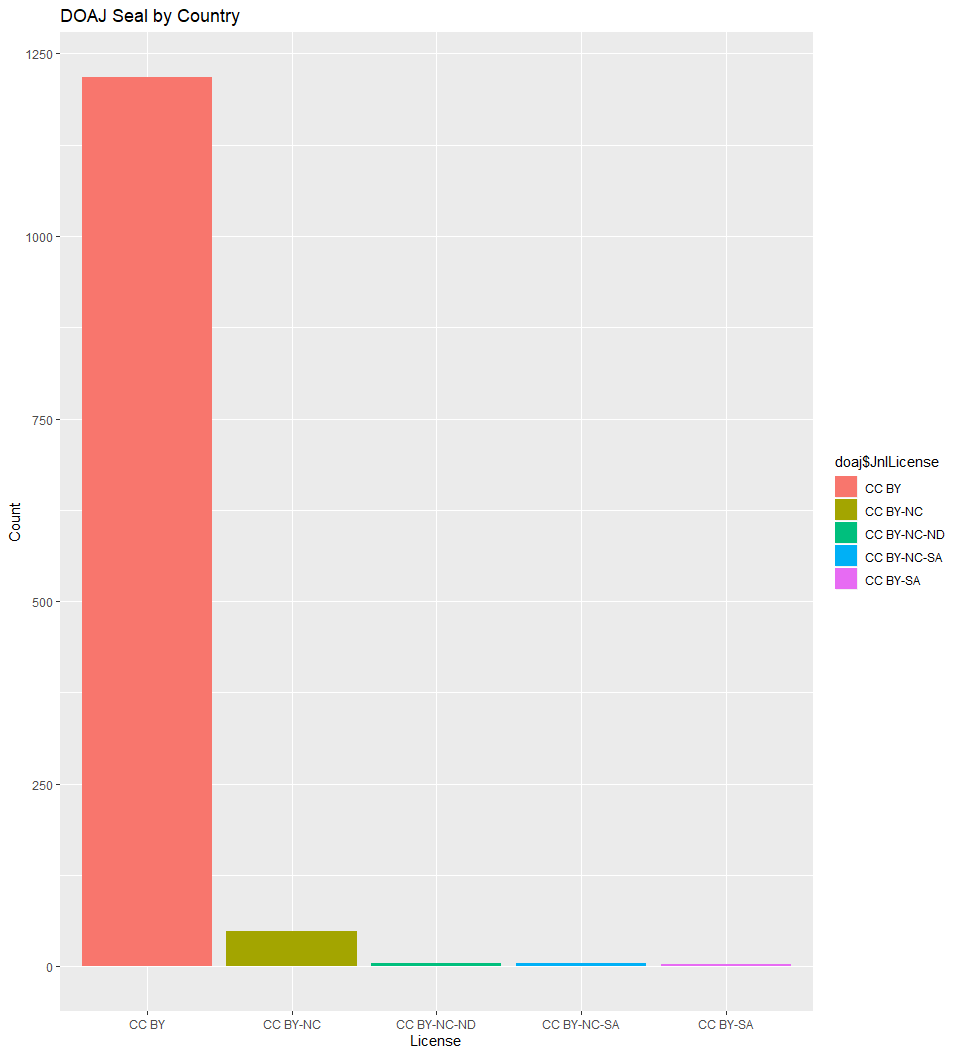
\includegraphics{Base_2013_1_files/figure-latex/plot_license-1.pdf}

\hypertarget{references}{%
\section*{References}\label{references}}
\addcontentsline{toc}{section}{References}

\hypertarget{refs}{}
\leavevmode\hypertarget{ref-Castro_2017}{}%
Castro, Eleni, Merc\e` Crosas, Alex Garnett, Kasey Sheridan, and Micah
Altman. 2017. ``Evaluating and Promoting Open Data Practices in Open
Access Journals.'' \emph{Journal of Scholarly Publishing} 49 (1).
University of Toronto Press Inc. (UTPress): 66--88.
\url{https://doi.org/10.3138/jsp.49.1.66}.

\leavevmode\hypertarget{ref-Vasilevsky_2017}{}%
``Reproducible and Reusable Research: Are Journal Data Sharing Policies
Meeting the Mark?'' n.d. 5. \url{https://doi.org/10.7717/peerj.3208}.


\end{document}
